% Insert one blank page after the thesis body, then start appendices.
\clearpage
\thispagestyle{empty}
\null
\clearpage

% Appendix labels:
% Appendix A, Appendix B, Appendix C
% Subsection numbering inside Appendix A: A.1, A.2, ...
\setcounter{section}{0}
\renewcommand{\thesubsection}{\Alph{section}.\arabic{subsection}}

\refstepcounter{section}
\section*{Appendix \Alph{section}: Guinness World Record Adjudication Rules and Logistical Framework}
\label{sec:appendix-a-gwr}

The computational optimization developed in this thesis is strictly bounded by the physical and logistical rules set forth by Guinness World Records (GWR) for the attempt ``Most countries visited in 24 hours by scheduled transport''. To ensure the mathematical model produced a legal, record-eligible sequence, the algorithm was calibrated against the official guidelines and direct clarifications from the GWR Records Management Team.

The core rules and their direct impacts on the routing model are as follows:
\begin{itemize}
  \item \textbf{Sovereign Definitions:} Eligible countries are strictly limited to the member states of the United Nations, Observer States, the Vatican, and Palestine. A ``visit'' is defined as physically setting foot within a country's borders, and each country is counted only once.
  \item \textbf{The ``Country 0'' Clock Initiation:} The GWR guidelines dictate that the continuous 24-hour clock starts the moment the challenger enters the first foreign country. The departure country does not count toward the total. Consequently, any initial domestic repositioning legs generated by the algorithm (e.g., a train to an airport within the starting country) were mathematically excluded from the final Route Quality Index (RQI) country tally.
  \item \textbf{Transport Modalities:} The attempt must be executed using only scheduled transport available to the general public. However, the GWR team clarified that walking and paid, receipt-logged taxi journeys are permitted specifically for connecting between public transport hubs. This ruling validated the algorithm's use of static walking and local-transit times to bridge unconnected aviation and rail hubs within the same city.
  \item \textbf{Airport Sovereignty:} GWR confirmed that passing passport control at an airport constitutes a valid sovereign visit, even if the challenger does not leave the terminal building. This validated the inclusion of airport nodes as sovereign endpoints in the directed graph, provided the participant obtains a physical passport stamp and timestamped photographic evidence.
  \item \textbf{Evidence Requirements:} The physical execution of the optimal route requires continuous GPS tracking (timestamped \texttt{.kml} files), the chronological retention of all original transit tickets and receipts, hourly updated witness logbooks, and unbroken, static video evidence of the entire 24-hour attempt.
\end{itemize}

\refstepcounter{section}
\section*{Appendix \Alph{section}: Label-Setting and Dynamic Programming Algorithms (AoE)}
\label{sec:appendix-b-algorithms}

This appendix contains the formal pseudocode for the algorithms developed during the evaluation of the Time-Dependent Activity-on-Edge (AoE) architecture discussed in Chapter 4. The algorithms are presented in their evolutionary order, demonstrating the progression from a naive baseline search to the final bi-directional stitching implementation.

\includepdf[pages=1,pagecommand={\noindent This naive approach forms the foundational dynamic programming search, relying solely on standard Pareto dominance without predictive bounding.\\[0.5\baselineskip]}]{../algorithms/development/algorithm_template.pdf}
\includepdf[pages=2,pagecommand={}]{../algorithms/development/algorithm_template.pdf}

\includepdf[pages=1,pagecommand={\noindent Introduces predictive pruning using precomputed reachable country sets to eliminate hopeless branches.\\[0.5\baselineskip]}]{../algorithms/development/algorithm_2.pdf}
\includepdf[pages=2,pagecommand={}]{../algorithms/development/algorithm_2.pdf}

\includepdf[pages=1,pagecommand={\noindent The precomputation step required for Algorithm 2. It calculates the $R(v,b)$ sets (reachable countries from node $v$ at time bucket $b$) via backward propagation.\\[0.5\baselineskip]}]{../algorithms/development/algorithm_3.pdf}

\includepdf[pages=1,pagecommand={\noindent Replaces the standard queue with a priority queue, scoring labels based on country count and time to aggressively expand promising nodes.\\[0.5\baselineskip]}]{../algorithms/development/algorithm_4.pdf}
\includepdf[pages=2,pagecommand={}]{../algorithms/development/algorithm_4.pdf}

\includepdf[pages=1,pagecommand={\noindent Calculates the absolute minimum time required to enter and exit each specific country's transit network to enable time-budgeted pruning.\\[0.5\baselineskip]}]{../algorithms/development/algorithm_5.pdf}

\includepdf[pages=1,pagecommand={\noindent Integrates the MTT precomputation (Algorithm 5) into the bounding logic to enforce physical time constraints on the theoretically reachable countries.\\[0.5\baselineskip]}]{../algorithms/development/algorithm_6.pdf}
\includepdf[pages=2,pagecommand={}]{../algorithms/development/algorithm_6.pdf}

\includepdf[pages=1,pagecommand={\noindent A rapid, randomized greedy probe designed to reach the 24-hour mark in milliseconds. It utilizes heavily biased weights for unvisited countries and a Tabu list to prevent local loops.\\[0.5\baselineskip]}]{../algorithms/development/algorithm_7.pdf}
\includepdf[pages=2,pagecommand={}]{../algorithms/development/algorithm_7.pdf}

\includepdf[pages=1,pagecommand={\noindent Integrates Algorithm 7 into the main queue expansion, triggering the rapid rollouts every 1,000 iterations to attempt early global record updates.\\[0.5\baselineskip]}]{../algorithms/development/algorithm_8.pdf}
\includepdf[pages=2,pagecommand={}]{../algorithms/development/algorithm_8.pdf}

\includepdf[pages=1,pagecommand={\noindent Introduces a GlobalMinTime constant to aggressively prune labels that mathematically lack the physical time required to bridge the gap between their current country count and the global record.\\[0.5\baselineskip]}]{../algorithms/development/algorithm_9.pdf}
\includepdf[pages=2-3,pagecommand={}]{../algorithms/development/algorithm_9.pdf}

\includepdf[pages=1,pagecommand={\noindent The first half of the bi-directional pivot. It executes the time-budgeted, hard-floor search strictly forward in time, terminating at the 14-hour mark to avoid nocturnal graph sparsity.\\[0.5\baselineskip]}]{../algorithms/development/algorithm_10.pdf}
\includepdf[pages=2,pagecommand={}]{../algorithms/development/algorithm_10.pdf}

\includepdf[pages=1,pagecommand={\noindent The second half of the bi-directional pivot. It evaluates the network in reverse, tracking inbound scheduled edges backward from the end of the 24-hour window, terminating at the 14-hour mark.\\[0.5\baselineskip]}]{../algorithms/development/algorithm_11.pdf}
\includepdf[pages=2,pagecommand={}]{../algorithms/development/algorithm_11.pdf}

\includepdf[pages=1,pagecommand={\noindent Evaluates the intersection of the forward and backward half-searches. It validates temporal continuity and geographic unions to reconstruct the globally optimal 24-hour path.\\[0.5\baselineskip]}]{../algorithms/development/algorithm_12.pdf}
\includepdf[pages=2,pagecommand={}]{../algorithms/development/algorithm_12.pdf}

\nopagebreak
\refstepcounter{section}
\section*{Appendix \Alph{section}: Temporal and Toponymic Normalization Dictionaries}
\label{sec:appendix-c-normalization-dictionaries}

This appendix details the explicit hardcoded dictionaries implemented within the data engineering pipeline to resolve upstream API inconsistencies, enforce deterministic UTC synchronization, and correct erroneous geographical assignments at complex European border crossings.

\subsection*{UTC Timezone Airport Overrides}
\label{subsec:appendix-c-utc-overrides}

While standard timezone synchronization relied on ISO alpha-2 country codes, outermost regions and non-contiguous territories required explicit IATA code overrides to prevent negative time-travel artifacts in the Directed Acyclic Graph. The following dictionary defines the specific offsets (in minutes) applied relative to UTC+0:

\begin{verbatim}
AIRPORT_OVERRIDES = {
    # UTC -1 (Azores)
    "PDL": -60, "TER": -60, "FLW": -60, "CVU": -60, "HOR": -60,
    "PIX": -60, "GRW": -60, "SJZ": -60, "SMA": -60,

    # UTC +0 (Canary Islands, Madeira, Faroe Islands, Crown Dependencies, Iceland)
    "LPA": 0, "TFS": 0, "TFN": 0, "ACE": 0, "FUE": 0, "SPC": 0, "VDE": 0, "GMZ": 0,
    "FNC": 0, "PXO": 0, "FAE": 0, "JER": 0, "GCI": 0, "IOM": 0, "ACI": 0,
    "AEY": 0, "EGS": 0, "GRY": 0, "IFJ": 0, "RKV": 0, "VPN": 0, "KEF": 0, "HFN": 0, "BIU": 0,

    # UTC +2 (Moldova)
    "RMO": 120, "KIV": 120,

    # UTC +3 (Turkey, Belarus, Western Russia)
    "IST": 180, "SAW": 180, "AYT": 180, "ESB": 180, "ADB": 180, "DLM": 180,
    "BJV": 180, "TZX": 180, "GZP": 180, "TEQ": 180, "SIP": 180,
    "MSQ": 180, "MVQ": 180, "BQT": 180, "GME": 180,
    "LED": 180, "SVO": 180, "DME": 180, "VKO": 180, "ZIA": 180,
    "AER": 180, "AAQ": 180, "KRR": 180, "ROV": 180, "VOZ": 180,

    # UTC +4 to +7 (Eastern Russian Hubs)
    "KUF": 240, "UFA": 300, "SVX": 300, "PEE": 300, "OVB": 420, "NOZ": 420, "KJA": 420
}
\end{verbatim}

\subsection*{Geopolitical Standardization and Border Corrections}
\label{subsec:appendix-c-geopolitical-corrections}

To ensure the multi-modal routing algorithm properly merged flight and rail data without fragmenting sovereign territories, geopolitical names were mapped to a unified standard. Additionally, stations situated near complex international borders whose administrative country differed from their linguistic profile were forcefully corrected using the following mappings.

\medskip
\textbf{Geopolitical Standardization:}

\begin{verbatim}
SPECIAL_COUNTRY_NAME_MAP = {
    "england": "GB",
    "scotland": "GB",
    "wales": "GB",
    "northern ireland": "GB",
    "united kingdom": "England", # Unified to match Deutsche Bahn nomenclature
    "moldova, republic of": "Moldova"
}
\end{verbatim}

\medskip
\textbf{Critical Border Station Corrections (Subset):}

\begin{verbatim}
STATION_CORRECTIONS = {
    "Genève, Mont-Blanc": "CH",        # Switzerland (Not France)
    "St-Léonard": "CH",                # Switzerland (Not France)
    "Bratislava hl.st.": "SK",         # Slovakia (Not Czechia)
    "Baden b.Wien": "AT",              # Austria (Not Germany)
    "Salzburg Liefering": "AT",        # Austria (Not Germany)
    "Ponte Gardena-Laion": "IT",       # Italy (Not Austria)
    "Domodossola": "IT",               # Italy (Border station)
    "Rybnik(CZ)": "PL",                # Poland (Not Czechia despite suffix)
    "Koebenhavns Lufthavn st": "DK",   # Denmark
    "Visby st": "SE",                  # Sweden (Not Denmark)
    "Komarom": "HU",                   # Hungary (Slovak side is Komárno)
    "Schaanwald, Zollamt": "LI"        # Liechtenstein (Not Switzerland)
}
\end{verbatim}
